\documentclass[11pt]{article}
\usepackage[a4paper,margin=2.4cm]{geometry}
\usepackage{booktabs,graphicx,amsmath,hyperref,xcolor}
\hypersetup{colorlinks,linkcolor=blue!50!black,citecolor=blue!50!black,urlcolor=blue!50!black}
\usepackage[numbers,sort&compress]{natbib}

\title{Where Should a RAG System Enforce Access Control?\\
\large Recall Loss, Shared-Statistics Leakage and Cache Leakage in Multi-Tenant Retrieval}
\author{Mithil Nagabathula\\University of East London\\\texttt{mithilnishu2000@gmail.com}}
\date{October 2026}

\begin{document}
\maketitle

\begin{abstract}
Retrieval-augmented generation (RAG) systems built for organisations must answer each user only from documents that user may see.
Implementations differ in where they enforce this: after retrieval (post-filtering), inside the search (pre-filtering), in separate
indexes per tenant, or not at all in an answer cache placed in front of the pipeline. We measure the consequences of each choice on a
multi-tenant version of the Reuters-21578 corpus (8{,}781 documents) with BM25 and dense retrieval.
Post-filtering a global top-\(k\) list silently lost relevant authorised documents: with dense retrieval, known-item recall in the
top 5 fell from 0.61 to 0.37, and fetching 16 times more candidates only recovered it to 0.59. Correct pre-filtering on a shared
index still leaked: because BM25 statistics were computed over all tenants, an attacker who could only upload documents and see the
order of their own results recovered the exact number of another tenant's documents containing a secret term in every one of 100
trials, using six queries. Per-tenant statistics removed the leak. A semantic answer cache keyed on query similarity alone served
unauthorised documents in about 90\% of its hits; adding the tenant to the key still left 27--30\% of hits leaking across roles, and
only keying on the user's full permission set removed the leak. By contrast, the number of results returned by a post-filtering system was not a useful existence oracle (AUC
0.50--0.53). We give a checklist for enforcement placement and release the code.
\end{abstract}

\section{Introduction}
Retrieval-augmented generation \cite{lewis2020rag} answers a question by retrieving documents and passing them to a language model.
In an organisation, documents carry permissions, and many products serve several customer organisations (tenants) from one
deployment. The question of \emph{where} to enforce permissions is usually answered for convenience: vector databases make it easy
to filter results after search, indexes are often shared to save cost, and semantic caches are added later for latency.

Each choice has a security and a quality consequence. Post-filtering can never return a forbidden document, but it can return fewer
or worse authorised ones. Pre-filtering returns the right documents, but scores may still depend on documents the user cannot see.
Caches keyed only on what was asked ignore who asked. Büttcher and Clarke showed two decades ago that shared term statistics in
multi-user desktop search leak information \cite{buttcher2005security}; RAG systems re-create the same architecture, and current
guidance lists vector and embedding weaknesses among the top risks for LLM applications \cite{owasp2025llm}. Prior RAG security work
has focused on extracting retrieved data through the model and on poisoning the corpus \cite{zeng2024ragprivacy,zou2025poisonedrag};
this paper looks one layer down, at the retrieval and caching layer, where the leaks are deterministic and the defences are cheap.

We contribute four measurements on a public corpus with synthetic permissions: (E1) the recall cost of post-filtering, (E2) whether
post-filtering leaks the existence of hidden documents through the result count, (E3) a rank-only attack on shared BM25 statistics
under correct pre-filtering, and (E4) leakage through a semantic answer cache.

\section{Setup}
\paragraph{Corpus and permissions.} We use the ApteMod split of Reuters-21578 \cite{apte1994reuters} distributed with NLTK
\cite{bird2009nltk}, keeping 8{,}781 articles with a headline of at least three words and a body of at least 20 words (86 topic
categories). Bodies are indexed; headlines serve as known-item queries, so the relevant document for a query is the article it heads.
Each document is assigned at random to one of \(T\) tenants (\(T\in\{2,4,8,16,32\}\)) and, within its tenant, is visible to all staff
(70\%), to one of four departments (20\%) or to executives only (10\%). A user belongs to one tenant and department and is an
executive with probability 0.2. Because permissions are random, any leak comes from the system design, not from the data.

\paragraph{Retrievers.} BM25 (\(k_1=1.2\), \(b=0.75\)) \cite{robertson2009bm25}, implemented so that the documents whose statistics feed
IDF and average length can be chosen independently of the documents that may be returned; and a dense retriever using 256-dimensional
latent semantic analysis embeddings \cite{deerwester1990lsa} with cosine similarity, a reproducible stand-in for a neural embedding
model. Answers use the top \(k=5\) documents.

\section{Results}
\subsection{E1: the recall cost of post-filtering}
A post-filtering system retrieves the global top \(fk\) and discards documents the user may not see; \(f\) is the over-fetch factor.
For each configuration we issued 600 queries (60 users, 10 authorised target documents each) over three random permission
assignments. Table~\ref{tab:postfilter} and Figure~\ref{fig:post} compare known-item recall with exact pre-filtering.

\begin{table}[t]
\centering
\caption{Known-item recall in the top 5 with exact pre-filtering and with post-filtering of a global top-$fk$ list, averaged over 2--32 tenants, 3 seeds and 600 user queries per setting. The last column is the share of queries for which post-filtering returned fewer than 5 documents.}
\label{tab:postfilter}
\small
\setlength{\tabcolsep}{4pt}
\begin{tabular}{lrrrrr}
\toprule
Retriever & Pre-filter & Post, 1$\times$ & Post, 4$\times$ & Post, 16$\times$ & Short answers at 4$\times$ \\
\midrule
BM25 & 0.774 & 0.706 & 0.755 & 0.770 & 70\% \\
Dense & 0.610 & 0.372 & 0.524 & 0.589 & 72\% \\
\bottomrule
\end{tabular}
\end{table}


\begin{figure}[t]
  \centering
  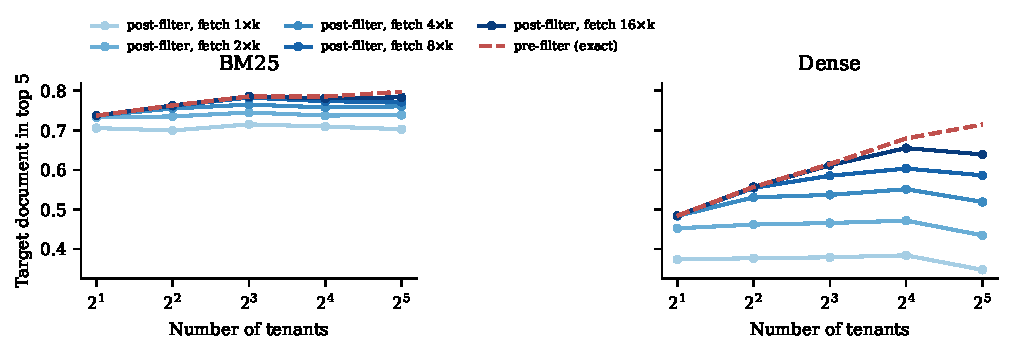
\includegraphics[width=\linewidth]{figures/postfilter.pdf}
  \caption{Known-item recall in the top 5 as the share of the index a user may see shrinks. Pre-filtering improves as the user's
  searchable corpus gets smaller; post-filtering does not, so the gap widens.}
  \label{fig:post}
\end{figure}

Post-filtering never returned a forbidden document, but it lost relevant authorised ones. Without over-fetching, recall fell from
0.774 to 0.706 with BM25 and from 0.610 to 0.372 with dense retrieval. The gap grew with the number of tenants: pre-filtering benefits
from a smaller effective corpus (dense recall rose from 0.48 with 2 tenants to 0.71 with 32), whereas post-filtered recall stayed near
0.37 throughout, because a user who can see 2\% of the index loses almost all of a global top-\(k\) list. Over-fetching helped but did
not close the gap: at \(f=16\), dense recall was 0.589 against 0.610. Post-filtered systems also returned short answer sets: at
\(f=4\), fewer than five documents came back for 70\% of queries. These failures are silent: the answer is simply worse.

\subsection{E2: does the result count reveal hidden documents?}
An outsider (a user of tenant 0) issued the headlines of documents they could not see (positives) and of documents not in the index
(negatives, a held-out 10\% of the corpus), and observed how many results came back. If hidden matches occupy slots in the global
top-\(fk\), positives should return fewer results. Across all configurations the AUC of this signal was 0.50--0.53 (mean 0.51): the
channel exists in principle but carried almost no information, because a user's own documents rarely fill the over-fetched list
anyway. We report this as a negative result; it does not make post-filtering safe, since E1's quality cost remains.

\subsection{E3: shared statistics leak through rankings}
Now assume correct pre-filtering: the attacker only ever sees their own documents. The index, however, is shared, and BM25's inverse
document frequency is computed over all tenants, as is the default in most search engines. The victim tenant holds \(m\in[0,40]\)
documents mentioning a secret term (a project code name, say). The attacker can upload documents to their own tenant and query. They
upload one probe document containing the secret term, and control documents containing fresh nonce terms, with exactly \(j\) copies for
nonce \(j\) (\(j=1,\dots,64\)), all of equal length. A query containing the secret term and nonce \(j\) ranks the probe above the control
exactly when the secret term is rarer than nonce \(j\), i.e.\ when \(m+1<j\). Binary search over \(j\) therefore recovers \(m\) from the
order of the attacker's own two documents.

\begin{figure}[t]
  \centering
  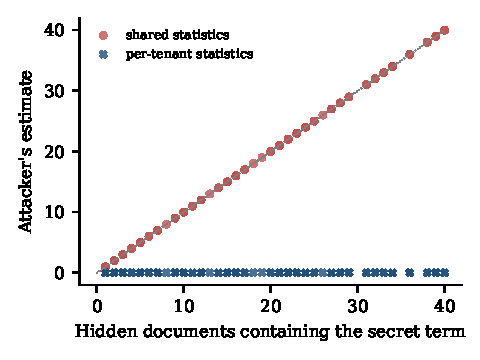
\includegraphics[width=0.55\linewidth]{figures/idf_attack.pdf}
  \caption{E3: the attacker's estimate of how many hidden documents contain the secret term, from rankings of their own documents only.}
  \label{fig:idf}
\end{figure}

With shared statistics the attack recovered \(m\) exactly in all 100 trials, using six queries each (Figure~\ref{fig:idf}). With
statistics computed only over the documents the user may see, the estimate was always zero and carried no information. The attack
needs neither scores nor any access to the victim's documents; it needs only the ability to add documents and observe order, which most
document-upload RAG products offer.

\subsection{E4: semantic answer caches}
\IfFileExists{tables/cache.tex}{\begin{table}[t]
\centering
\caption{A semantic answer cache over 10{,}000 paraphrased queries from 400 users in 8 tenants. An answer leaks if it contains a document the asking user may not see.}
\label{tab:cache}
\small
\setlength{\tabcolsep}{4pt}
\begin{tabular}{llrrr}
\toprule
Cache key & Threshold & Hit rate & Leaking answers & Share of hits that leak \\
\midrule
query only & 0.85 & 82.6\% & 74.4\% & 90.1\% \\
query only & 0.95 & 73.6\% & 66.4\% & 90.3\% \\
query + tenant & 0.85 & 63.2\% & 18.7\% & 29.5\% \\
query + tenant & 0.95 & 51.1\% & 13.8\% & 27.0\% \\
query + permission set & 0.85 & 41.4\% & 0.0\% & 0.0\% \\
query + permission set & 0.95 & 30.0\% & 0.0\% & 0.0\% \\
\bottomrule
\end{tabular}
\end{table}
}{}
A semantic cache \cite{bang2023gptcache} returns a stored answer when a new query's embedding is within a similarity threshold of an
earlier one. We simulated 10{,}000 queries from 400 users in 8 tenants: popular questions (2{,}000 headlines with Zipf-distributed
popularity) asked in paraphrased form (random word dropout and swaps). An answer is the set of documents retrieved for the user who
first asked; a later hit returns it unchanged. We compared three cache keys: the query alone, the query plus tenant, and the query plus
the user's full permission set (tenant, department and executive flag), across thresholds from 0.80 to 0.98 (Table~\ref{tab:cache}).

A cache keyed on the query alone served unauthorised documents in about 90\% of hits at every threshold, so 62--78\% of all answers
contained documents the user could not see. Raising the threshold reduced hits but not the share of hits that leaked. Adding the tenant
to the key cut leakage to 12--20\% of answers, but did not remove it: within a tenant, departments and executives see different
documents, and 27--30\% of hits still crossed those boundaries. Keying on the full permission set removed leakage entirely, at the
cost of a lower hit rate (41\% against 63\% at a threshold of 0.85), because users who share a permission set can still share answers.

\section{Discussion}
\paragraph{A placement checklist.}
(1) Enforce permissions \emph{inside} retrieval (pre-filtering), never only afterwards; if a vector store forces post-filtering, measure
recall against a pre-filtered baseline and over-fetch accordingly. (2) Compute ranking statistics per tenant, or use a scoring function
that does not depend on other tenants' documents; for dense retrieval, fit any corpus-level components (such as vocabularies or
normalisers) per tenant. (3) Key any answer or retrieval cache on the full permission context of the user, not on the tenant alone.
(4) Test these properties with canary documents, as in E3, as part of a release process.

\paragraph{Limitations.} Permissions were random rather than drawn from a real organisation; correlated permissions would change E1's
magnitude but not its direction. Dense retrieval used LSA rather than a neural embedding model, whose corpus-level dependence is
weaker (embeddings do not depend on other documents) but whose approximate-nearest-neighbour indexes raise the same post-filtering
issue. We did not include a language model, so leaks that the model itself might add or mask are out of scope. E3 assumes the attacker
can upload documents and that the system reports results in rank order.

\section{Conclusion}
Where access control is enforced in a RAG system changes both its quality and its security. Post-filtering silently reduced recall,
shared BM25 statistics let a tenant count another tenant's secret documents from rankings alone, and permission-blind caches served
unauthorised documents. Each problem has a simple fix that costs little when designed in.

\paragraph{Reproducibility.} Code and results will be released at
\newline\url{https://github.com/mithil2k2000-tech/rag-access-control-study}.

\paragraph{Use of AI tools.} An AI assistant (Claude, Anthropic) helped write experiment code and draft text. The author designed the
study questions, reviewed the code and results, and takes responsibility for the content.

\bibliographystyle{plainnat}
\bibliography{refs}
\end{document}
